\section{Problems}

\subsection{Question One}

The following shows a history of customers with their incomes, age groups, and an attribute called Have\_iPhone indicating whether they have an iPhone. We also indicate whether they will buy an iPad or not in the last column. We want to use Naive Bayes to predict whether a new customer will buy an iPad or not. Consider a new young customer whose income is medium and who has an iPhone. Please predict whether this new customer will buy an iPad.

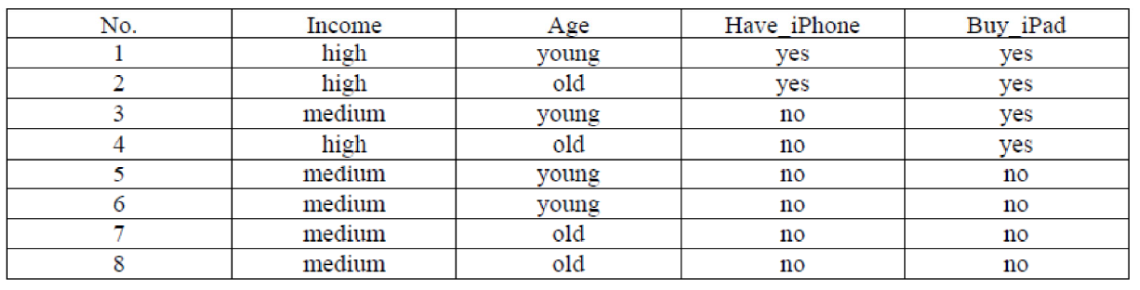
\includegraphics[width=1\textwidth]{media/hw5_q1.png}

For each attribute: medium income ($I=m$), young age ($A=y$), have iPhone ($iPhone=y$) for our new customer, let's calculate the probability for each value of buying an iPad (yes, no). We do this by counting the number of matching attribute values for each possible value of `Buy\_iPad' (yes, no).
\begin{align}
    P(I=m | iPad = y) &= \frac{1}{4} \label{eq:q1_1} \nonumber \\
    P(I=m | iPad = n) &= \frac{4}{4} = 1
\end{align}
\begin{align}
    P(A=y | iPad = y) &= \frac{2}{4} = \frac{1}{2}\label{eq:q1_2} \nonumber \\
    P(A=y | iPad = n) &= \frac{2}{4} = \frac{1}{2}
\end{align}
\begin{align}
    P(iPhone=y | iPad = y) &= \frac{2}{4} = \frac{1}{2}\label{eq:q1_3} \nonumber \\
    P(iPhone=y | iPad = n) &= \frac{0}{4} = 0
\end{align}

We also calculate the total probability of `Buy\_iPad':
\begin{align}
    P(iPad = y) &= \frac{4}{8} = \frac{1}{2}\label{eq:q1_4} \nonumber \\
    P(iPad = n) &= \frac{4}{8} = \frac{1}{2}
\end{align}

Finally we use Bayes' rule and for each value of `Buy\_iPad', calculate the class probability, given the customer's attributes:
\begin{align}
    P(iPad = y|\text{attributes}) &= P(iPad = y)\cdot P(I=m | iPad = y) \cdot P(A=y | iPad = y) \cdot P(iPhone=y | iPad = y) \label{eq:q1_5} \nonumber \\
    &= \frac{1}{2} \cdot \frac{1}{4} \cdot \frac{1}{2} \cdot \frac{1}{2} \nonumber \\
    &= 0.03125
\end{align}
\begin{align}
    P(iPad = n|\text{attributes}) &= P(iPad = n)\cdot P(I=m | iPad = n) \cdot P(A=y | iPad = n) \cdot P(iPhone=y | iPad = n) \label{eq:q1_6} \nonumber \\
    &= \frac{1}{2} \cdot 1 \cdot \frac{1}{2} \cdot 0 \nonumber \\
    &= 0
\end{align}

Finally, we compare the calculated class probabilities (Eq. \ref{eq:q1_5} vs \ref{eq:q1_6}) given the attributes:
\begin{align}
    [P(iPad = n|\text{attributes}) = 0.03125] &> [P(iPad = n|\text{attributes}) = 0]
\end{align}

$\therefore$ This new customer with the given attributes: medium income ($I=m$), young age ($A=y$), have iPhone ($iPhone=y$), \textbf{is likely} to buy an iPad with 0.03125 probability.

\subsection{Question Two}
You have been asked to develop a classification model for diagnosing whether a patient is infected with a certain disease. To help you construct the models, your collaborator has provided you with a small training set (N=10 individuals) with equal number of positive and negative examples. You tried several approaches and found two most promising models, C1 and C2. The outputs of the models in terms of predicting whether each of the training examples belong to the “positive(+)” class are summarized in the table below. The first row shows the probability a training example belongs to the positive class according to the classifier C1, while the second row shows the same information for classifier C2. The last row indicates the true class labels of the 10 training examples.

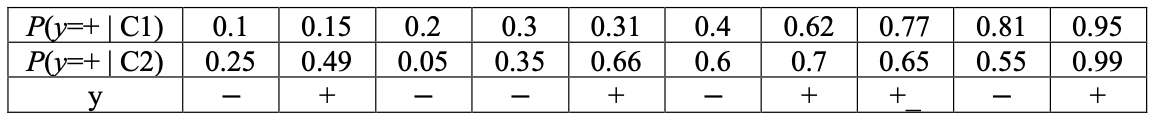
\includegraphics[width=1\textwidth]{media/hw5_q2.png}

For each model, we will evaluate different thresholds within the range of [0,1], and a sample with probability P(y=+ | C1) (or P(y=+ | C2)) that is lower than this threshold will be estimated as -, or + if greater than this threshold. By varying the thresholds (referred to the lecture slide on ROC), you can study the model performance and draw the ROC. (you can either use code or hand-calculating, but if you use code, you need to show the calculation process.)

\textbf{a. Draw the corresponding ROC curves for each classifier on the same plot.}

I wrote some code to do this, the code is included in the Jupyter notebook. Here are the resulting ROC curves for each classifier C1 and C2:

\begin{figure}[h]
    \centering
    \begin{minipage}{0.49\textwidth}
        \centering
        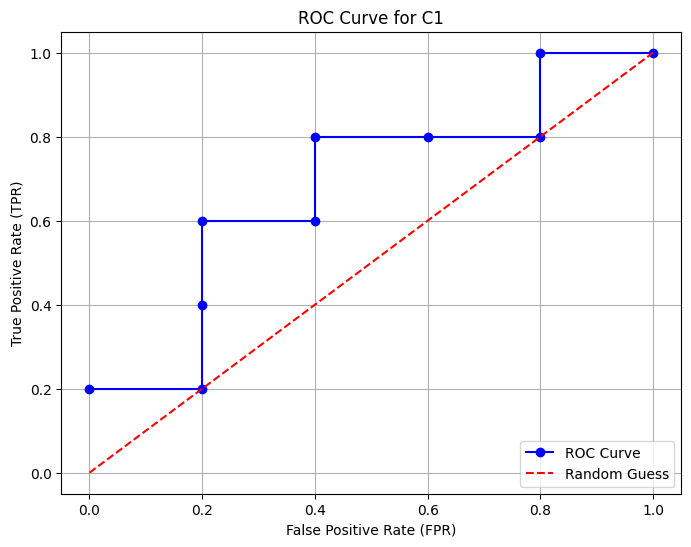
\includegraphics[width=\textwidth]{media/hw5_q1_c1.png}
        \caption{ROC Curve for classifier C1.}
    \end{minipage}
    \hfill
    \begin{minipage}{0.49\textwidth}
        \centering
        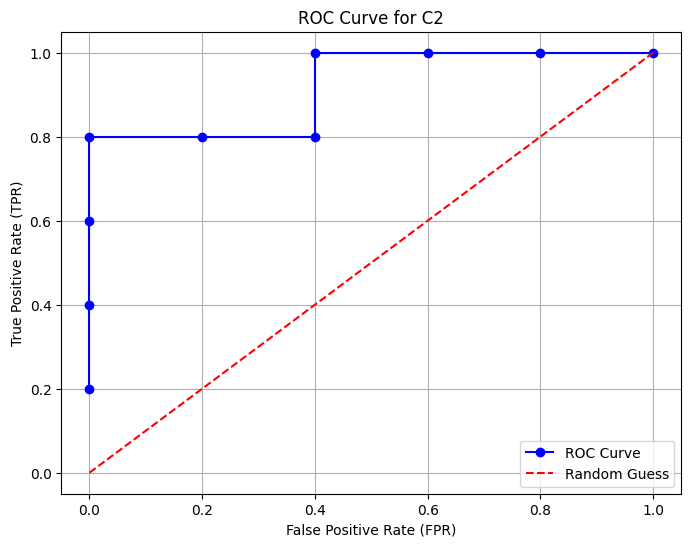
\includegraphics[width=\textwidth]{media/hw5_q1_c2.png}
        \caption{ROC Curve for classifier C2.}
    \end{minipage}
\end{figure}


\textbf{b. Which classifier can be considered better? Why?}
